\chapter{Sets, Functions, and Relations}
\pagebreak[4]

\section{Sets and Membership }
\subsection{}
\begin{tcolorbox}
List explicitly the elements of the set 
$$\{x:\,x<0 \text{ and } (x-1)(x+2)(x+3)=0\}$$
\end{tcolorbox}
$$\{\,-3,\, -2\}$$
$$\blacklozenge$$

\subsection{}
\begin{tcolorbox}
List the elements of the set 
$$\{x:\,3x-1  \text{ is a multiple of  } 3\}$$
\end{tcolorbox}
$$\{x:\,x= k+\frac{1}{3},\, k\in \mathbb{Z}\}$$
$$\blacklozenge$$
\subsection{}
\begin{tcolorbox}
Sketch on a number line each of the following sets.\\
(a) $\{x:\,|x-1| \leq 3  \}$\\
(b) $\{x:\,|x-1| \leq 3 \text{ and } |x| \leq 2 \}$\\
(c) $\{x:\,|x-1| \leq 3 \text{ or } |x| \leq 2 \}$
\end{tcolorbox}
\begin{figure}[H]%
    \centering
    \subfloat[]{\input{./images/fig_1.1.3_a.tex}}\\
    \subfloat[]{\input{./images/fig_1.1.3_b.tex}}\\
    \subfloat[]{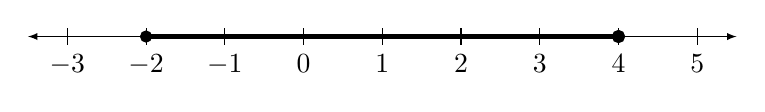
\begin{tikzpicture}
\draw[ultra thick] (-2,0) -- (4,0);
\path [draw=black, fill=black] (-2,0) circle (2pt);
\path [draw=black, fill=black, thick] (4,0.0) circle (2pt);
\draw[latex-latex, very thin] (-3.5,0) -- (5.5,0) ;
\foreach \x in  {-3,-2,-1,0,1,2,3,4,5}
\draw[shift={(\x,0)},color=black] (0pt,3pt) -- (0pt,-3pt);
\foreach \x in {-3,-2,-1,0,1,2,3,4,5}
\draw[shift={(\x,0)},color=black] (0pt,0pt) -- (0pt,-3pt) node[below] 
{$\x$};
\end{tikzpicture}}\\
%\caption{}
\label{fig:fig_p3}
\end{figure}
$$\blacklozenge$$
\newpage
\section{Some remarks on the use of the connectives \textit{and, or, implies}}
\subsection{}
\begin{tcolorbox}
Demonstrate by means of a table showing truth values that the following is a true statement for any choice of $p$ and $q$. Thus show that it is a tautology.
$$(\lnot q\Rightarrow \lnot p)\Rightarrow ( p \Rightarrow q)$$
\end{tcolorbox}
\begin{displaymath}
\begin{array}{|c c|c c|c|c|c|}
% |c c|c| means that there are three columns in the table and
% a vertical bar ’|’ will be printed on the left and right borders,
% and between the second and the third columns.
% The letter ’c’ means the value will be centered within the column,
% letter ’l’, left-aligned, and ’r’, right-aligned.
p & q &\lnot q &\lnot p &\lnot q\Rightarrow \lnot p& p\Rightarrow q&(\lnot q\Rightarrow \lnot p)\Rightarrow ( p \Rightarrow q) \\ % Use & to separate the columns
\hline % Put a horizontal line between the table header and the rest.
T & T &F&F& T&T&T\\
T & F &T&F& F&F&T\\
F & T &F&T& T&T&T\\
F & F &T&T& T&T&T\\
\end{array}
\end{displaymath}
$$\blacklozenge$$

\subsection{}
\begin{tcolorbox}
Show by means of a truth table  that the statement 
$$((p\Rightarrow q) \wedge (q\Rightarrow r))\Rightarrow (p\Rightarrow r)$$
is a tautology.
\end{tcolorbox}
\begin{displaymath}
\begin{array}{|c c c|c| c|c|c|c|}
p & q &r & p\Rightarrow q &q\Rightarrow r &(p\Rightarrow q) \wedge (q\Rightarrow r))& p\Rightarrow r&((p\Rightarrow q) \wedge (q\Rightarrow r))\Rightarrow (p\Rightarrow r)\\ % 
\hline 
T & T &T&T&T& T&T&T\\
T & T &F&T&F& F&F&T\\
T & F &T&F&T& F&T&T\\
T & F &F&F&T& F&F&T\\
F & T &T&T&T& T&T&T\\
F & T &F&T&F& F&T&T\\
F & F &T&T&T& T&T&T\\
F & F &F&T&T& T&T&T\\
\end{array}
\end{displaymath}
$$\blacklozenge$$
\subsection{}
\begin{tcolorbox}
Show by means of a truth table  that  
$$(p\wedge q) \Rightarrow (p\vee q)$$
is a tautology.
\end{tcolorbox}
\begin{displaymath}
\begin{array}{|c c|c|c|c|}
p & q &p\wedge q& p\vee q&(p\wedge q) \Rightarrow (p\vee q) \\ 
\hline 
T & T & T&T&T\\
T & F & F&F&T\\
F & T & F&T&T\\
F & F & F&F&T\\
\end{array}
\end{displaymath}
$$\blacklozenge$$
\subsection{}
\begin{tcolorbox}
Suppose that $p$ and $q$ are statements such that $(p \wedge q)$ is a false statement. Does it follow that the statement
$$(p\text{ is false}) \vee (q\text{ is false})$$is a true statement?
\end{tcolorbox}
\begin{displaymath}
\begin{array}{|c c|c|c c| c|}
p & q &p\wedge q& \lnot p&\lnot q& \lnot p \vee \lnot q\\ % Use & to separate the columns
\hline % Put a horizontal line between the table header and the rest.
T & F & F&F&T&T\\
F & T & F&T&F&T\\
F & F & F&T&T&T\\
\end{array}
\end{displaymath}
\textbf{The answer is Yes}.
$$\blacklozenge$$

\subsection{}
\begin{tcolorbox}
Negate the following statement: \textit{If two angles of a triangle have equal measure, then the length of two sides of that triangle are equal.}
\end{tcolorbox}
First we note that $\lnot(p\Rightarrow q)\Leftrightarrow (p \wedge \lnot q)$. Indeed,

\begin{displaymath}
\begin{array}{|c c|c|c | c|c| c|}

p & q &p\Rightarrow q& \lnot(p\Rightarrow q)&\lnot q&p \wedge \lnot q &\lnot(p\Rightarrow q)\Leftrightarrow (p \wedge \lnot q)\\ % Use & to separate the columns
\hline % Put a horizontal line between the table header and the rest.
T & T & T&F&F&F&T\\
T & F & F&T&T&T&T\\
F & T & T&F&F&F&T\\
F & F & T&F&T&F&T\\
\end{array}
\end{displaymath}
Putting $p$ as \textit{two angles of a triangle have equal measure} and $\lnot q$ as \textit{no two sides of that triangle have equal length} we get the true 'false' statement:\\
\textbf{Two angles of a triangle have equal measure} $\wedge$  \textbf{no two sides of that triangle have equal length}. 
$$\blacklozenge$$

\subsection{}
\begin{tcolorbox}
Write the contrapositive of the statement in Exercise 5.
\end{tcolorbox}
The contrapositive of $p\Rightarrow q$ is $\lnot q\Rightarrow \lnot p$.
Putting $\lnot p$ as \textit{no two angles of a triangle have equal measure} and $\lnot q$ as \textit{no two sides of that triangle have equal length} we get \\
\textbf{If no two sides of that triangle have equal length then no two angles of a triangle have equal measure.}
$$\blacklozenge$$

\subsection{}
\begin{tcolorbox}
Write the converse of the statement in Exercise 5.
\end{tcolorbox}
The converse of $p\Rightarrow q$ is $q\Rightarrow  p$,  giving \\
\textbf{If two sides of a triangle have equal length then  two angles of a that triangle have equal measure.}
$$\blacklozenge$$

\subsection{}
\begin{tcolorbox}
Write the contrapositive of the following statement\\
\textit{If a person belongs to Committee A, then he must be a member of Committee B and he must be a member of Committee C.}
\end{tcolorbox}
Lets put 
\begin{align*}
p\equiv \text{a person belongs to Committee A}\\
q\equiv \text{a person belongs to Committee B}\\
r\equiv \text{a person belongs to Committee C}\\
\end{align*}
then the given statement translates as 
$$p\Rightarrow (q\wedge r)$$

and the contrapositive 
$$\lnot (q\wedge r)\Rightarrow \lnot p$$
This last statement is equivalent with 
$$(\lnot q\vee \lnot r)\Rightarrow \lnot p$$ or in plain text:\\
\textbf{If a person does not belong to Committee B or C , then he is not  a member of Committee A.}
$$\blacklozenge$$

\subsection{}
\begin{tcolorbox}
Write the contrapositive of the following statement\\
$$\text{If } x\in A \text{ and } x\in B\text{, then } x \in C$$
\end{tcolorbox}
Lets put 
\begin{align*}
p\equiv x\in A\\
q\equiv x\in B\\
r\equiv x\in C\\
\end{align*}
then the given statement translates as 
$$p\wedge r\Rightarrow r$$

and the contrapositive 
$$\lnot (r)\Rightarrow \lnot (p\wedge q)$$
This last statement is equivalent with 
$$\lnot (r)\Rightarrow (\lnot p\vee \lnot q)$$ i.e:\\
$$x\notin C \Rightarrow (x\notin A \vee x\notin B)$$
$$\blacklozenge$$
\newpage
\section{Subsets}
\section{Union and Intersection of sets}
\subsection{}
\begin{tcolorbox}

\end{tcolorbox}

$$\blacklozenge$$